\chapter{Lección 1: Temas de teoría de cuerdas}

\lectureoverview{El desafío al reduccionismo se agudiza con la bosonización en \(1+1\) dimensiones, la dualidad eléctrica--magnética, las D-branas, las transiciones de acoplamiento fuerte, la geometría emergente y el paisaje combinatorio de los vacíos de la teoría de cuerdas. Un mismo sistema físico puede admitir descripciones elementales radicalmente distintas; cuál de ellas parece sencilla depende del acoplamiento y de la geometría.}

\section{Reduccionismo, complejidad y la cuestión de la simplicidad}

Susskind comienza con un lema filosófico deliberadamente familiar: las cosas grandes están hechas de cosas pequeñas, y las pequeñas, de otras aún más pequeñas. Luego añade la versión más ambiciosa de la misma idea, la que de verdad importa para la física fundamental: al descender por capas cada vez más profundas, los objetos deberían volverse no solo más pequeños, sino también más simples. Su metáfora es que las casas están hechas de ladrillos y que nadie confunde una casa con un ladrillo. El ladrillo es más pequeño, pero también más simple.

El primer paso de la lección consiste en contrastar esa expectativa con la situación real de la física de partículas. Si el reduccionismo estuviera conduciendo a una simplicidad cada vez mayor en ese sentido fuerte, cabría esperar que la física actual de partículas elementales fuera bastante parca. Sin embargo, Susskind recalca que, incluso antes de que entre en juego la gravedad cuántica, las cuentas ya son engorrosas. En la lección se trata de cifras aproximadas, pero esa imprecisión forma parte del argumento:
\begin{equation}
\begin{aligned}
N_{\mathrm{species}}&\sim 75,\\
N_{\mathrm{independent}}&\sim 10\text{--}20,\\
N_{\mathrm{parameters}}&\sim 20.
\end{aligned}
\end{equation}
Y eso ni siquiera pone fin a la historia. El Modelo Estándar no incluye la gravedad, no explica la materia oscura, no aporta la estructura adicional necesaria para la inflación y presenta un grave problema de ajuste fino. Añadir los mecanismos correctivos habituales solo aumenta el recuento. La supersimetría es el ejemplo que da la lección. En la época de la lección, muchos físicos esperaban que el Gran Colisionador de Hadrones revelara supercompañeros; Susskind subraya que la extensión correspondiente introduciría más de cien parámetros adicionales, en vez de simplificar de inmediato las cuentas. Su mensaje esquemático es
\begin{equation}
N_{\mathrm{parameters}}^{\mathrm{extended}} \sim 200.
\end{equation}
Estas cifras son deliberadamente aproximadas y propias de la época. Sirven para apoyar el argumento de que una descripción más profunda no tiene por qué parecer más sencilla si se cuentan las partículas y las constantes medidas.

Esta objeción cuantitativa todavía no es la tesis principal de Susskind. Es solo el preludio. La afirmación más profunda, que impulsa el resto de la lección, es que la teoría cuántica de campos moderna y la teoría de cuerdas no respaldan de manera evidente una distinción única, independiente del acoplamiento, entre los ladrillos y las casas. Los ejemplos siguientes muestran que el propio significado de ``elemental'' puede depender de cuáles sean las variables más eficaces.

\section{Bosonización: primer quiebre de una fundamentabilidad fija}

El primer ejemplo teórico de Susskind proviene de una teoría cuántica de campos en \(1+1\) dimensiones: una dimensión espacial y una temporal. Anuncia de inmediato que no va a derivar la equivalencia en detalle; lo importante no es la demostración formal, sino la enseñanza conceptual.

Se parte de una teoría de campos de fermiones. El campo fermiónico se denota por \(\psi\). Dos fermiones cercanos pueden formar un compuesto bosónico, y el campo bosónico correspondiente se denota por \(\phi\). A primera vista, la jerarquía parece clara: \(\psi\) es fundamental, mientras que \(\phi\) es una variable compuesta o efectiva. En la lección, el bosón se introduce precisamente así: como un campo que crea pares ligados de fermiones.

Sin embargo, se descubrió que la misma teoría puede reformularse partiendo del punto de vista opuesto. Se puede comenzar con el campo bosónico \(\phi\), y entonces el fermión deja de aparecer como un constituyente puntual. En cambio, aparece como un kink del campo bosónico: una configuración extendida en la que \(\phi\) interpola suavemente entre dos valores asintóticos. El contenido matemático mínimo que presenta la lección es esta estructura asintótica:
\begin{equation}
\phi(x\to -\infty)=\phi_-,
\qquad
\phi(x\to +\infty)=\phi_+.
\end{equation}
Una forma esquemática representativa y conveniente es
\begin{equation}
\phi(x)\approx \frac{\phi_++\phi_-}{2}
+
\frac{\phi_+-\phi_-}{2}\tanh\!\left(\frac{x}{\ell}\right),
\end{equation}
donde \(\ell\) es la anchura de la región de transición.

\editorialnote{El perfil de tangente hiperbólica es una forma suave estándar de representar el kink que aparece en el dibujo de la lección; no se deriva allí como fórmula. El diccionario preciso de bosonización depende del modelo; la idea conceptual es el intercambio entre una excitación fermiónica y un solitón topológico de un campo bosónico.}

La analogía de la correa que presenta la lección es lo bastante precisa como para conservarla. Una correa plana y sin torsión es una configuración sin kink. Si se gira un extremo en \(2\pi\), lejos de allí la correa vuelve a tener la misma orientación local, pero entre ambos extremos debe atravesar una región retorcida y extendida. Esa región retorcida es el kink. En la descripción bosónica, el fermión está representado precisamente por un objeto extendido de ese tipo.

La idea se vuelve más clara al introducir un acoplamiento. En este ejemplo, Susskind lo llama \(G\). No se trata de que las dos descripciones estén relacionadas vagamente, sino de que su eficacia depende del régimen del parámetro:
\begin{align}
G \ll 1
&\Rightarrow
\ell\text{ small, tight kink; }\psi\text{ efficient},\\
G \gg 1
&\Rightarrow
\ell\text{ large, broad kink; }\phi\text{ efficient}.
\end{align}
Para valores pequeños de \(G\), el kink es estrecho y el fermión parece el objeto sencillo. A medida que aumenta \(G\), el kink se ensancha y el fermión se vuelve menos puntual. Entonces, las variables bosónicas resultan más económicas.

\paragraph{Esquema del procedimiento.}
\begin{enumerate}
\item Partir de una teoría fermiónica descrita por \(\psi\).
\item Identificar los compuestos bosónicos descritos por \(\phi\).
\item Reformular toda la misma teoría en términos de \(\phi\).
\item En la descripción bosónica, el fermión reaparece como un kink de anchura \(\ell\).
\item Para \(G\ll 1\), \(\ell\) es pequeño y la descripción fermiónica es la más sencilla.
\item Para valores mayores de \(G\), \(\ell\) aumenta y la descripción bosónica pasa a ser la más sencilla.
\end{enumerate}

Este es el primer contraejemplo explícito a la imagen fija de las ``casas y los ladrillos''. La conclusión de la lección no es simplemente que existan objetos compuestos, sino que lo que cuenta como variable elemental puede cambiar con el acoplamiento.

\section{Carga eléctrica, monopolos magnéticos y acoplamiento débil frente a fuerte}

A continuación, Susskind pregunta si aparece una historia análoga en una física de partículas más familiar. El ejemplo contrapone la carga eléctrica al monopolo magnético. En este lenguaje, una partícula cargada ordinaria, como el electrón, es un monopolo eléctrico: una fuente localizada de campo eléctrico. El monopolo magnético se introduce mediante la analogía de una barra imantada. Si de algún modo se pudiera aislar el extremo de una barra imantada sin la barra que lo conecta y que no se ve, las líneas de campo serían exactamente como las de una carga eléctrica, pero magnéticas en vez de eléctricas.

El parámetro de control pertinente es la constante de estructura fina \(\alpha\). En la lección, Susskind la trata heurísticamente como el cuadrado de la carga eléctrica:
\begin{equation}
\alpha \sim e^2.
\end{equation}
También ofrece una interpretación operacional aproximada: mide con qué facilidad radia un electrón, y resume la intensidad diciendo que un electrón acelerado radia del orden de ``\(1/100\)'' fotones en el sentido pertinente. En los propios términos numéricos aproximados de la lección,
\begin{equation}
\alpha \approx 10^{-2}.
\end{equation}
No se pretende establecer una convención precisa, sino expresar pedagógicamente que la carga eléctrica es débil.

\editorialnote{La relación débil--fuerte tiene un antecedente preciso en la cuantización de Dirac. En una convención habitual, las cargas eléctrica y magnética satisfacen \(e g_m=2\pi n\). Así, un acoplamiento eléctrico débil corresponde a uno magnético fuerte, aunque los factores numéricos exactos y las relaciones de masas protegidas dependen de la teoría.}

Cuando \(\alpha\ll 1\), el electrón es el objeto sencillo. Su campo eléctrico es débil, su nube de polarización del vacío es tenue y parece casi puntual. El monopolo magnético es entonces lo contrario: su campo es enorme, su entorno está muy distorsionado y es extenso, complejo y pesado. Susskind resume la situación precisamente en estos términos de acoplamiento débil--fuerte:
\begin{equation}
\begin{aligned}
\alpha \ll 1
&\Rightarrow \text{simple electron;}\\
&\phantom{\Rightarrow{}}\text{heavy, extended monopole},\\
\alpha \gg 1
&\Rightarrow \text{simple monopole;}\\
&\phantom{\Rightarrow{}}\text{heavy, structured electron}.
\end{aligned}
\end{equation}
La lección no deriva una fórmula para la masa del monopolo. No hace falta. La idea es cualitativa. A medida que aumenta \(\alpha\), el campo del electrón se intensifica y su estructura crece, mientras que el monopolo se contrae y se vuelve más ligero. Muy por encima de la unidad, se intercambian las descripciones útiles: el monopolo es sencillo y el electrón, complejo.

Esta es la versión de teoría de campos de la lección anterior sobre bosonización. La distinción entre lo fundamental y lo compuesto no es absoluta. Depende del acoplamiento.

\begin{classroomqa}
\audiencequestion{Si el reduccionismo no es una guía fiable, ¿por qué los físicos se basan en el cálculo, que parece dividir un sistema en partes arbitrariamente pequeñas? \lecturetimestamp{00:21:21}}
\lecturerresponse{El cálculo afirma que las variaciones son suaves; no identifica los objetos fundamentales de una teoría. Los campos cuánticos fluctúan a todas las escalas de distancia, lo que produce una jerarquía interminable, en lugar de una capa final y suave en la que se pueda decidir de una vez por todas qué es elemental.}
\end{classroomqa}

El intercambio continúa con la sugerencia de que la jerarquía se parece a un fractal. Susskind acepta la analogía y luego la precisa: los campos cuánticos fluctúan a todas las escalas, así que nunca son suaves en el sentido clásico. Esta variación excesiva es parte de lo que hace matemáticamente difícil la teoría cuántica de campos; el cálculo ordinario debe aplicarse a magnitudes renormalizadas, no a un campo microscópico ingenuamente suave.

\section{Cuerdas, D-branas y el retorno de la dualidad débil--fuerte}

La siguiente transición de la lección es deliberadamente ingenua. Si la teoría de cuerdas ha de ser la teoría de los bloques fundamentales, la respuesta debería ser sencilla: los bloques fundamentales son cuerdas. Susskind enuncia abiertamente esa expectativa y luego dedica la parte siguiente de la lección a desarmarla.

\subsection{Por qué las cuerdas no son toda la historia}

La primera complicación es la presencia inevitable de las D-branas. Una D\(p\)-brana es un objeto de \(p\) dimensiones en el que pueden terminar las cuerdas. La letra \(D\) proviene de las condiciones de contorno de Dirichlet, pero el nombre importa mucho menos que su función: estos objetos forman parte de la teoría y no se pueden descartar. No son adornos opcionales.

Los ejemplos más sencillos son:
\begin{itemize}
\item una D0-brana, que es puntual,
\item una D1-brana, o cuerda D, que tiene forma de cuerda,
\item una cuerda F, la cuerda fundamental ordinaria.
\end{itemize}
Una D0-brana es un sitio puntual y pesado en el que puede terminar cualquier número de cuerdas F. Una D1-brana es un objeto pesado, parecido a un cable, mucho más grueso y con más masa por unidad de longitud que una cuerda F, pero también puede servir de punto de terminación para las cuerdas F. La lección no presenta estos objetos como alternativas igualmente elementales cuando el acoplamiento es débil. Introduce las D-branas como objetos pesados, estructurados y de aspecto compuesto que, sin embargo, la teoría nos obliga a incluir.

\editorialnote{La teoría de branas impares que se usa en esta parte de la lección es la teoría de cuerdas de tipo IIB. Sus D-branas estables tienen dimensión espacial impar, incluidas las D1-branas y las D3-branas. Susskind pospone estos nombres porque el tema inmediato es el patrón de dualidad, no la clasificación.}

\paragraph{Notación.}
Susskind usa \(G\) y \(g\) con cierta flexibilidad en distintas partes de la lección. Aquí se reserva \(G\) para el ejemplo de bosonización, mientras que \(g\) denota el acoplamiento de cuerdas.

El acoplamiento de cuerdas \(g\) se define operacionalmente, no axiomáticamente. Es el parámetro que mide la probabilidad de que una cuerda fluctuante se divida y forme cuerdas hijas. Por eso Susskind lo compara directamente con la función de \(\alpha\) en la electrodinámica cuántica. La lección también se detiene a identificar la tensión con la energía por unidad de longitud:
\begin{equation}
T=\frac{E}{L}=\frac{M}{L}.
\end{equation}

Para una cuerda F y una cuerda D, las fórmulas habituales de la tensión hacen explícita la comparación entre acoplamiento débil--y fuerte:
\begin{equation}
T_{\mathrm{F1}}=\frac{1}{2\pi\alpha'},
\qquad
T_{\mathrm{D1}}=\frac{1}{2\pi\alpha' g_s},
\qquad
\frac{T_{\mathrm{D1}}}{T_{\mathrm{F1}}}=\frac{1}{g_s}.
\end{equation}
\editorialnote{Estas fórmulas de la tensión proporcionan la normalización convencional que subyace a la comparación cualitativa de la lección entre cables e hilos. Son una adición editorial; en la lección solo se usa la dependencia con el acoplamiento.}

\subsection{Cuerdas F y cuerdas D}

El mismo relato débil--fuerte vuelve a aparecer en el lenguaje de las cuerdas. A acoplamiento pequeño, la cuerda F es ligera, delgada y se acerca a la imagen intuitiva original del objeto fundamental. La cuerda D es gruesa, pesada y está llena de estructura de cuerdas F. Al aumentar el acoplamiento, la cuerda F se divide con mayor facilidad; la nube de cuerdas hijas prolifera a su alrededor y la cuerda se vuelve más pesada y complicada. Al mismo tiempo, a la cuerda D le resulta cada vez más difícil emitir las cuerdas F, ahora pesadas, por lo que su estructura circundante se vuelve más tenue y la cuerda, más ligera y parecida a una línea. Así pues, la correspondencia débil--fuerte de la conferencia es
\begin{align}
g \ll 1
&\Rightarrow
\begin{gathered}
\text{F-string light and thin;}\\
\text{D-string heavy and structured},
\end{gathered}\\
g \sim 1
&\Rightarrow
\text{F-string and D-string comparable},\\
g \gg 1
&\Rightarrow
\begin{gathered}
\text{D-string light and thin;}\\
\text{F-string heavy and structured}.
\end{gathered}
\end{align}
Susskind señala que, alrededor de \(g\sim 1\), las dos descripciones dejan de distinguirse con claridad. A partir de ahí, en la práctica, intercambian sus papeles. Esta es la versión en teoría de cuerdas del intercambio electrón--monopolo, y su nombre aceptado es dualidad S.

Se puede seguir el mismo intercambio cuando una cuerda se cierra formando un lazo. Con acoplamiento débil, un pequeño lazo de cuerda F es una excitación ligera, similar a una partícula, mientras que el lazo de cuerda D correspondiente es pesado y complejo. Con acoplamiento fuerte, sus funciones se invierten: el lazo de cuerda D pasa a ser la descripción ligera, y entre las excitaciones ligeras de cuerda cerrada resultantes se encuentra el gravitón. La lección usa este ejemplo para insistir en que incluso la identidad de una partícula conocida puede depender del lado de la dualidad que se use.

La lección lleva la idea un paso más allá. En la teoría idealizada, el acoplamiento no es simplemente un número que se ajusta a mano; se comporta como un campo. Esquemáticamente,
\begin{equation}
g = g(x).
\end{equation}
Por tanto, distintas regiones del espacio pueden favorecer descripciones duales distintas. En una región, las cuerdas F son las variables ligeras; en otra, lo son las cuerdas D. Entre ambas, nada es especialmente sencillo. Por eso, para Susskind, la teoría de cuerdas no restablece la imagen reduccionista sencilla. Radicaliza la ambigüedad.

\editorialnote{En la teoría de cuerdas perturbativa, el acoplamiento local viene determinado por el dilatón, \(g_s(x)=e^{\Phi(x)}\). Por tanto, escribir \(g=g(x)\) no es una mera analogía, aunque las compactificaciones realistas suelen generar un potencial que restringe estas variaciones.}

\begin{classroomqa}
\audiencequestion{Si el acoplamiento variara lo suficiente como para que las cuerdas D fueran más ligeras que las cuerdas F en otra región, ¿afectaría ese cambio a los espectros observables? \lecturetimestamp{00:34:15}}
\lecturerresponse{Sí. Esa es una de las razones por las que el modelo exactamente simétrico y controlable matemáticamente que se está tratando no se puede identificar directamente con nuestro mundo. Sus enseñanzas se refieren a lo que pueden hacer las teorías cuánticas consistentes, no a un espectro literal de la naturaleza.}
\end{classroomqa}

\begin{classroomqa}
\audiencequestion{¿Existe una descripción dual análoga para una D2-brana? \lecturetimestamp{00:34:39}}
\lecturerresponse{Sí, pero no consiste en otro intercambio parecido al de las cuerdas D. El caso de branas pares conducirá a una interpretación mediante membranas y a una dimensión espacial adicional; esa es la siguiente construcción.}
\end{classroomqa}

\begin{classroomqa}
\audiencequestion{¿Una probabilidad mayor de que una cuerda se divida explica el aumento de la complejidad interna? \lecturetimestamp{00:34:53}}
\lecturerresponse{Sí. Para concretar el mecanismo, volvamos a la electrodinámica cuántica: un electrón emite fotones, los fotones fluctúan y producen pares cargados, y esas líneas cargadas vuelven a radiar. Al aumentar el acoplamiento, esa jerarquía se vuelve menos tenue.}
\end{classroomqa}

\subsection{Vuelta a la electrodinámica cuántica a partir de una pregunta}

A continuación, un estudiante pregunta si una probabilidad mayor de división significa simplemente una estructura más compleja ``a monte.'' Susskind responde volviendo a la electrodinámica cuántica y dibujando de nuevo la línea de universo del electrón. Esta vuelta es importante: muestra que la historia de las cuerdas no es una curiosidad aislada, sino otro caso del mismo patrón de acoplamiento débil--fuerte.

\begin{figure}[htbp]
\centering
\begin{tikzpicture}[scale=1.0]
\draw[->] (-1.2,0) -- (3.7,0) node[right] {space};
\draw[->] (0,-0.2) -- (0,4.3) node[above] {time};

\draw[line width=0.9pt] (0,0.2) -- (0,4.0);
\node[left] at (0,3.55) {\(e^{-}\)};

\draw[line width=0.8pt] (0,1.0) -- (0.18,1.08) -- (0.36,0.92) -- (0.54,1.10) -- (0.72,0.94) -- (0.90,1.12) -- (1.08,0.96) -- (1.26,1.14);
\draw[line width=0.8pt] (0,2.35) -- (-0.18,2.43) -- (-0.36,2.27) -- (-0.54,2.45) -- (-0.72,2.29) -- (-0.90,2.47);

\draw[line width=0.8pt] (1.26,1.14) -- (1.48,1.42);
\draw[line width=0.8pt] (1.26,1.14) -- (1.04,1.42);
\draw[line width=0.8pt] (1.48,1.42) -- (1.58,2.10);
\draw[line width=0.8pt] (1.04,1.42) -- (0.94,2.10);
\draw[line width=0.8pt] (0.94,2.10) -- (1.58,2.10);

\draw[line width=0.7pt] (1.58,1.78) -- (1.72,1.84) -- (1.86,1.72) -- (2.00,1.86);
\draw[line width=0.7pt] (0.94,1.78) -- (0.80,1.84) -- (0.66,1.72) -- (0.52,1.86);

\node at (2.35,1.95) {\(\gamma\)};
\node at (-1.15,2.75) {\(\gamma\)};
\end{tikzpicture}
\caption{Jerarquía esquemática de la electrodinámica cuántica que se usa en la lección: un electrón puntual emite fotones, los fotones crean pares y las líneas cargadas hijas vuelven a radiar, produciendo estructura a escalas cada vez menores.}
\end{figure}

La idea de la lección es que incluso un electrón puntual está acompañado por una jerarquía de procesos:
\begin{enumerate}
\item un electrón emite y absorbe fotones,
\item un fotón puede crear un par de electrón--positrón,
\item las líneas cargadas hijas pueden emitir fotones,
\item la jerarquía continúa a escalas menores.
\end{enumerate}
Con acoplamiento débil, esta nube es tenue, así que en el laboratorio el electrón parece casi puntual. Con un acoplamiento más fuerte, la nube se multiplica y el electrón se convierte en un objeto estructurado. La historia de las cuerdas se presenta entonces como un análogo directo de esta.

La misma discusión posterior también sirve de base para el balance heurístico de energía de Susskind. Insiste en que la energía pertinente no es simplemente la suma de las contribuciones de las partículas libres. También hay que incluir la energía de interacción:
\begin{equation}
E_{\mathrm{tot}} = E_e + E_\gamma + E_{\mathrm{int}}.
\end{equation}
Aquí, \(E_{\mathrm{int}}\) es el término crucial. Permite que la masa del electrón vestido incluya la energía asociada a su campo circundante y a su estructura virtual. La lección no convierte esto en una derivación formal de la autoenergía renormalizada. La idea es heurística, pero esencial: la masa del objeto ya incluye la energía de interacción necesaria para sostener la compleja nube que lo rodea.

\begin{classroomqa}
\audiencequestion{¿De dónde proviene la energía de los fotones virtuales y de los pares de electrón--positrón si un electrón no tiene suficiente energía libre para crear un par real? \lecturetimestamp{00:37:01}}
\lecturerresponse{Nunca se parte de un electrón desnudo para añadirle después su campo de Coulomb. El electrón observado es un estado vestido, y su masa ya incluye la energía del campo y la energía de interacción. En la electrodinámica cuántica, la energía total no es solo la energía del electrón libre más la del fotón libre; el término de interacción es indispensable. Es útil llamar virtuales a los pares intermedios, pero el balance de energía corresponde al estado interactuante completo.}
\end{classroomqa}

\begin{classroomqa}
\audiencequestion{Cuando una sonda de alta energía revela esta estructura, ¿la ha creado la sonda en vez de descubrir algo que ya estaba presente? \lecturetimestamp{00:38:59}}
\lecturerresponse{Esa distinción interpretativa se puede debatir. Desde el punto de vista operacional, la dispersión a energías suficientemente altas tiene un estado final calculable y no trivial. Con acoplamiento débil, la mayoría de los sucesos siguen pareciendo sencillos, mientras que una fracción del orden de \(\alpha\) revela radiación o pares adicionales.}
\end{classroomqa}

\begin{classroomqa}
\audiencequestion{Cuando se dice que la D1-brana tiene más masa que la cuerda F, ¿también es mayor su tensión? \lecturetimestamp{00:39:37}}
\lecturerresponse{Sí. Para una cuerda extendida, aquí ``masa'' significa energía por unidad de longitud, que es precisamente la tensión.}
\end{classroomqa}

\begin{figure}[htbp]
\centering
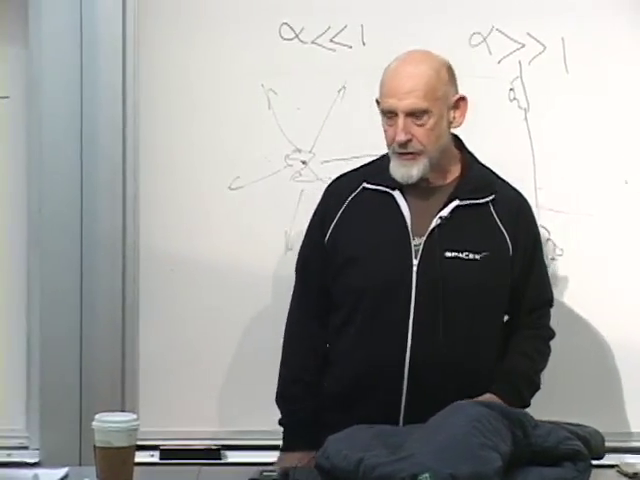
\includegraphics[width=0.72\textwidth]{lecture_01_figure_02.png}
\lectureframe{00:38:22.500}

\vspace{1em}

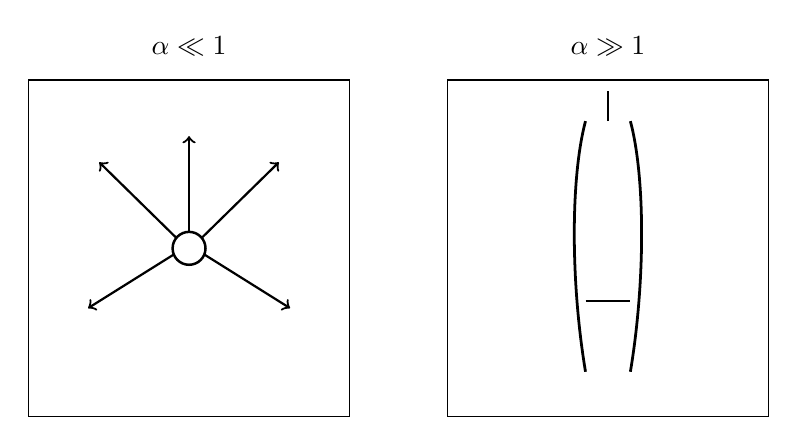
\begin{tikzpicture}[scale=0.95]
\draw (-5.3,-2.4) rectangle (-1.0,2.1);
\draw (0.3,-2.4) rectangle (4.6,2.1);

\node at (-3.15,2.55) {$\alpha \ll 1$};
\node at (2.45,2.55) {$\alpha \gg 1$};

\draw[line width=0.9pt] (-3.15,-0.15) circle (0.22);
\draw[->,line width=0.8pt] (-3.15,0.07) -- (-3.15,1.35);
\draw[->,line width=0.8pt] (-2.98,-0.01) -- (-1.95,1.00);
\draw[->,line width=0.8pt] (-3.32,-0.01) -- (-4.35,1.00);
\draw[->,line width=0.8pt] (-2.95,-0.23) -- (-1.80,-0.95);
\draw[->,line width=0.8pt] (-3.35,-0.23) -- (-4.50,-0.95);

\draw[line width=1.0pt] (2.15,-1.8) .. controls (1.95,-0.6) and (1.95,0.8) .. (2.15,1.55);
\draw[line width=1.0pt] (2.75,-1.8) .. controls (2.95,-0.6) and (2.95,0.8) .. (2.75,1.55);
\draw[line width=0.8pt] (2.15,-0.85) -- (2.75,-0.85);
\draw[line width=0.8pt] (2.45,1.55) -- (2.45,1.95);
\end{tikzpicture}
\caption{Comparación entre acoplamiento débil--fuerte en la electrodinámica cuántica, durante la discusión de la energía de interacción. El diagrama aísla los dos regímenes que Susskind presenta: una nube tenue con acoplamiento débil y otra que se multiplica con acoplamiento fuerte.}
\end{figure}

La razón por la que esta figura aparece aquí, aunque la comparación entre acoplamiento débil--y fuerte se introdujo antes, es que en la lección Susskind vuelve a dibujar el contraste más adelante, al responder preguntas sobre la energía de interacción y la estructura que se multiplica.

\section{Teorías de branas pares y dimensión adicional emergente}

Hasta aquí, la lección ha desarrollado con fuerza la idea del intercambio: fermión frente a bosón, electrón frente a monopolo, cuerda F frente a cuerda D. El paso siguiente es más sorprendente. Susskind pasa a otra versión de la teoría de cuerdas, con D-branas de dimensión par en lugar de impar. La distinción importa porque en esta teoría no hay una cuerda D que intercambiar con la cuerda F. Hay D0-branas, D2-branas, D4-branas y así sucesivamente.

Por tanto, el límite de acoplamiento fuerte no puede consistir simplemente en cambiarle el nombre a una cuerda por el de otra. Según la lección, ocurre algo más extraño: se hace manifiesta una dimensión espacial adicional. Susskind lo enuncia deliberadamente primero de la forma más dramática --- ``aparece una nueva dimensión'' --- y enseguida lo reformula con más cuidado: una dirección compacta muy pequeña se expande hasta que ya no se puede ignorar.

El recuento forma parte de la idea, así que se detiene a examinarlo:
\begin{equation}
\begin{aligned}
10\text{-dimensional string theory} &= 9\text{ space}+1\text{ time},\\
11\text{-dimensional theory} &= 10\text{ space}+1\text{ time}.
\end{aligned}
\end{equation}
La afirmación de la lección es que el límite de acoplamiento fuerte de la teoría de branas pares es efectivamente undimensional.

\editorialnote{La teoría de branas pares es la teoría de cuerdas de tipo IIA, y su compleción a acoplamiento fuerte es la teoría M. En unidades estándar, el radio del círculo emergente y la longitud de Planck undimensional escalan como \(R_{11}=g_s\ell_s\) y \(\ell_{11}=g_s^{1/3}\ell_s\). Estos nombres y fórmulas hacen explícito el diccionario moderno que subyace a la descripción geométrica de la lección.}

\subsection{El sándwich de mantequilla de cacahuete}

Para imaginar la dirección compacta, Susskind usa el modelo del ``sándwich de mantequilla de cacahuete'': dos láminas de pan infinitamente delgadas, con espacio real entre ellas. La regla especial es que al salir por un lado se vuelve por el otro. En una notación convencional que la lección describe de forma pictórica, no formal, se puede escribir
\begin{equation}
y \sim y + 2\pi R.
\end{equation}
Si \(R\) es muy pequeño, los observadores que viven en el sándwich describen efectivamente su mundo como de menor dimensión. Entonces, el cambio clave a acoplamiento fuerte es
\begin{equation}
g\uparrow
\qquad \Longrightarrow \qquad
R_{\mathrm{compact}}\uparrow.
\end{equation}
Eso es lo que quiere decir Susskind cuando afirma que aparece una nueva dimensión espacial: no que el espacio se cree de la nada, sino que una dirección compacta antes diminuta se expande y se vuelve visible en la teoría efectiva.

\begin{figure}[htbp]
\centering
\resizebox{\linewidth}{!}{%
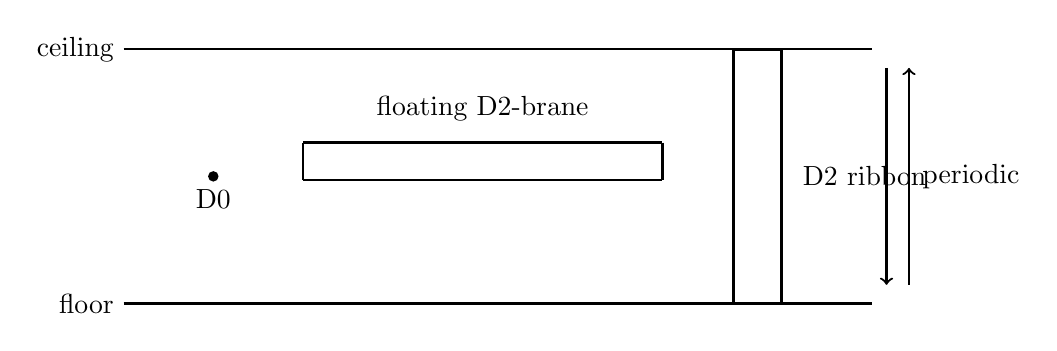
\begin{tikzpicture}[scale=0.95]
\draw[line width=0.9pt] (-5,1.7) -- (5,1.7);
\draw[line width=0.9pt] (-5,-1.7) -- (5,-1.7);

\node[left] at (-5,1.7) {ceiling};
\node[left] at (-5,-1.7) {floor};

\draw[->,line width=0.8pt] (5.2,1.45) -- (5.2,-1.45);
\draw[->,line width=0.8pt] (5.5,-1.45) -- (5.5,1.45);
\node[right] at (5.55,0) {periodic};

\draw[line width=1.0pt] (-2.6,0.45) -- (2.2,0.45);
\draw[line width=1.0pt] (-2.6,-0.05) -- (2.2,-0.05);
\draw[line width=1.0pt] (-2.6,0.45) -- (-2.6,-0.05);
\draw[line width=1.0pt] (2.2,0.45) -- (2.2,-0.05);
\node at (-0.2,0.9) {floating D2-brane};

\draw[line width=1.0pt] (3.15,-1.7) -- (3.8,-1.7);
\draw[line width=1.0pt] (3.15,1.7) -- (3.8,1.7);
\draw[line width=1.0pt] (3.15,-1.7) -- (3.15,1.7);
\draw[line width=1.0pt] (3.8,-1.7) -- (3.8,1.7);
\node[right] at (3.95,0) {D2 ribbon};

\fill (-3.8,0) circle (0.07);
\node[below] at (-3.8,-0.05) {D0};
\end{tikzpicture}
}%
\caption{La compactificación en forma de sándwich. Los bordes superior e inferior están identificados periódicamente; una D2-brana flota entre ellos como una alfombra, mientras que otra se extiende del suelo al techo y parece una cuerda cuando la dirección compacta es pequeña.}
\end{figure}

\subsection{¿Qué ocurre con las D0- y las D2-branas?}

La lección pregunta ahora qué ocurre con las D0-branas y las cuerdas. La respuesta no es simétrica. A medida que \(g\) aumenta, las D0-branas se vuelven cada vez más ligeras; en la interpretación de dimensión superior, se incorporan a la torre de partículas que llevan momento en la dirección recién manifiesta. Así, un objeto pesado y complejo en la descripción de acoplamiento débil se convierte en una excitación ligera ordinaria en la descripción de acoplamiento fuerte.

La relación entre las masas muestra la identificación:
\begin{equation}
M_{D0}(n)=\frac{n}{g_s\ell_s}
=\frac{n}{R_{11}}
=M_{\mathrm{KK}}(n).
\end{equation}
\editorialnote{Susskind llama a las D0-branas ``los gravitones'' de la teoría undimensional. Más precisamente, sus estados ligados son los modos de momento de Kaluza--Klein del multiplete de supergravedad undimensional, cuyo sector sin masa contiene el gravitón. Esta distinción conserva la identificación física de la lección y evita afirmar literalmente que se trata de una sola partícula.}

Las D2-branas explican el destino de las cuerdas. En la lección se destacan dos configuraciones:
\begin{enumerate}
\item una D2-brana que flota entre el suelo y el techo, como una alfombra en la mantequilla de cacahuete;
\item una D2-brana que se extiende del suelo al techo como una cinta, extendida a lo largo de la dirección visible.
\end{enumerate}
Cuando el sándwich es delgado, la cinta parece efectivamente unidimensional. Es el objeto que los observadores de baja energía llaman cuerda. A medida que se abre la dirección compacta, ese mismo objeto se vuelve inequívocamente parecido a una membrana. Como ahora ocupa más espacio en la dirección vertical, se vuelve pesado y deja de parecer una cuerda.

\paragraph{La lógica de la transición.}
\begin{enumerate}
\item Partimos de una dirección compacta muy pequeña, de modo que la cinta que va del suelo al techo se comporta, en la práctica, como una cuerda.
\item Aumentamos \(g\) y la dirección compacta se expande.
\item Las D0-branas se vuelven ligeras y se reinterpretan como estados de momento de Kaluza--Klein en la teoría de dimensiones superiores.
\item La cinta de D2-brana, que parecía una cuerda, se convierte en una membrana visiblemente extendida y se vuelve pesada.
\end{enumerate}
Este es el punto de inflexión de la lección: de la dualidad a la geometría emergente. El acoplamiento fuerte no se limita a intercambiar un objeto por otro; cambia cuál es la geometría más conveniente para describir el sistema.

Susskind se detiene en lo extraño que suena todo esto. La red de identificaciones propuestas exigía difíciles relaciones de consistencia matemática; algunas de ellas primero se presentaron a los físicos como conjeturas y luego fueron demostradas por matemáticos. No afirma que se conozca cada vacío realista de la teoría de cuerdas, sino que la propia red de dualidades ha superado pruebas de rigor inusualmente exigente.

Si el acoplamiento varía de un lugar a otro en este marco idealizado, la geometría más conveniente también puede variar. Una región puede parecer casi de diez dimensiones, con cuerdas ligeras y D0-branas pesadas; otra puede abrirse a la descripción de once dimensiones, con membranas enrolladas pesadas y modos de Kaluza--Klein ligeros. El cambio local de lenguaje forma parte de la misma red de dualidades.

La transcripción recoge brevemente el nombre de estas relaciones como ``desigualdades.'' Por el contexto, la palabra que se quería decir es \emph{dualidades}: relaciones entre extremos opuestos del espacio de parámetros. La corrección importa porque la conclusión de la lección es precisamente que no se conoce una lista única de constituyentes fundamentales. Las cuerdas, las branas, las partículas y la geometría de dimensiones superiores pueden transformarse unas en otras; o bien ningún elemento de la red es absolutamente fundamental, o bien existe una organización más profunda que aún se desconoce.

\section{D3-branas, membranas enrolladas y una imagen geométrica de la dualidad}

Tras la pausa, Susskind describe explícitamente el tema como una ``enorme red'' de teorías e ideas interconectadas. Los siguientes ejemplos no son nuevos efectos aislados, sino puentes que enlazan los anteriores.

\subsection{La variedad de mundo de una D3-brana}

El primer puente se construye con una D3-brana. Una D3-brana tiene tres dimensiones espaciales, y un observador confinado en ella podría confundirla fácilmente con el espacio ordinario. La brana puede curvarse y fluctuar, mientras que las cuerdas que terminan en ella pueden unirse, dividirse y dispersarse. Para un observador que solo ve las direcciones a lo largo de la brana, cada extremo parece una partícula, y las interacciones entre los extremos, una teoría cuántica de campos ordinaria.

\begin{figure}[htbp]
\centering
\resizebox{\linewidth}{!}{%
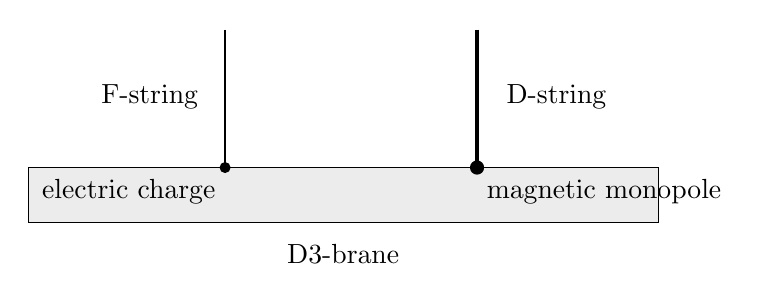
\begin{tikzpicture}[scale=1.0]
\draw[fill=gray!15] (-4,-0.35) rectangle (4,0.35);
\node at (0,-0.75) {D3-brane};

\draw[line width=0.9pt] (-1.5,2.1) -- (-1.5,0.35);
\fill (-1.5,0.35) circle (0.07);
\node[left] at (-1.72,1.25) {F-string};
\node[below left] at (-1.5,0.32) {electric charge};

\draw[line width=1.5pt] (1.7,2.1) -- (1.7,0.35);
\fill (1.7,0.35) circle (0.09);
\node[right] at (1.95,1.25) {D-string};
\node[below right] at (1.7,0.32) {magnetic monopole};
\end{tikzpicture}
}%
\caption{Interpretación en términos de la variedad de mundo de una D3-brana. El extremo de una cuerda F aparece como una carga eléctrica; el extremo de una cuerda D, como un monopolo magnético.}
\end{figure}

Esta es una de las identificaciones más satisfactorias de la lección. Para un observador en la variedad de mundo, una cuerda F que termina en la D3-brana aparece como una carga eléctrica. Una cuerda D que termina en esa misma brana aparece como un monopolo magnético. En otras palabras, la dualidad entre las cuerdas F y D se convierte, en la variedad de mundo de la D3-brana, en la dualidad eléctrica--magnética de la teoría de campos ordinaria. Lo que antes era una analogía ahora es un diccionario explícito.

\editorialnote{Para una pila de D3-branas, la descripción de baja energía en el volumen de mundo es la teoría de Yang--Mills supersimétrica en cuatro dimensiones \(\mathcal N=4\). Su dualidad eléctrica--magnética es la realización en teoría de campos de la S-dualidad de la teoría de tipo IIB; una sola brana da el límite abeliano que se usa de forma pictórica en la clase.}

\subsection{Dos direcciones compactas y enrollamientos asimétricos}

Susskind vuelve entonces a la geometría de dimensiones superiores y compactifica no una, sino dos direcciones pequeñas. Como no se pueden dibujar once dimensiones en una pizarra, comprime en una sola dirección horizontal visible las siete direcciones grandes que no aparecen en el esquema y dibuja explícitamente las dos compactas. Insiste en representar la compactificación de forma asimétrica, porque una dirección compacta debe ser más corta que la otra para que las cuerdas efectivas tengan tensiones distintas.

\begin{figure}[htbp]
\centering
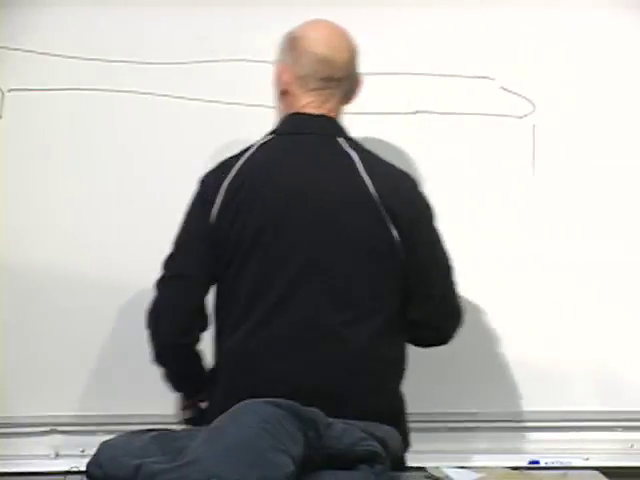
\includegraphics[width=0.78\textwidth]{lecture_01_figure_03.png}
\lectureframe{01:10:25.000}
\caption{Configuración final en la pizarra para las dos membranas enrolladas. Los ciclos compactos corto y largo producen las cintas similares a cuerdas F y D dibujadas a la derecha.}
\end{figure}

Una membrana puede enrollarse alrededor de cualquiera de las dos direcciones compactas y parecer una cuerda desde las direcciones no compactas. Si \(R_1\) y \(R_2\) son los radios de los dos círculos, sus tensiones efectivas son
\begin{equation}
\begin{aligned}
T_{(1)}&=2\pi R_1 T_{\mathrm{M2}},\\
T_{(2)}&=2\pi R_2 T_{\mathrm{M2}},\\
\frac{T_{(1)}}{T_{(2)}}&=\frac{R_1}{R_2}.
\end{aligned}
\end{equation}
Así, tamaños distintos de los círculos producen tensiones distintas para las cuerdas. Si identificamos el enrollamiento más corto con la cuerda F ligera y el más largo con la cuerda D pesada, podemos escribir esquemáticamente
\begin{equation}
g_s\sim \frac{R_{\mathrm{short}}}{R_{\mathrm{long}}},
\qquad
\frac{T_{\mathrm{D1}}}{T_{\mathrm{F1}}}\sim \frac{1}{g_s}.
\end{equation}

\begin{classroomqa}
\audiencequestion{¿Puede entenderse el acoplamiento de esta imagen como la razón entre las dos dimensiones compactas? \lecturetimestamp{01:10:13}}
\lecturerresponse{Sí. El parámetro de acoplamiento débil--fuerte se expresa geométricamente como una razón de aspecto. Si se hace corta una dirección, el acoplamiento se vuelve pequeño; intercambiar las dos direcciones intercambia las cuerdas ligera y pesada.}
\end{classroomqa}

\editorialnote{En la lección se llama provisionalmente \(\alpha\) a esta razón, reutilizando el símbolo que antes se había usado para la constante de estructura fina de la electrodinámica cuántica. Aquí escribimos \(g_s\) para mantener separados ambos significados. En la construcción completa de la teoría M, el acoplamiento de tipo IIB está codificado en la estructura compleja del toro compacto de dos dimensiones; el numerador preciso depende de cómo se etiqueten sus ciclos.}

La imagen de la membrana enrollada puede resumirse sin la distorsión de perspectiva del dibujo en la pizarra:

\begin{figure}[htbp]
\centering
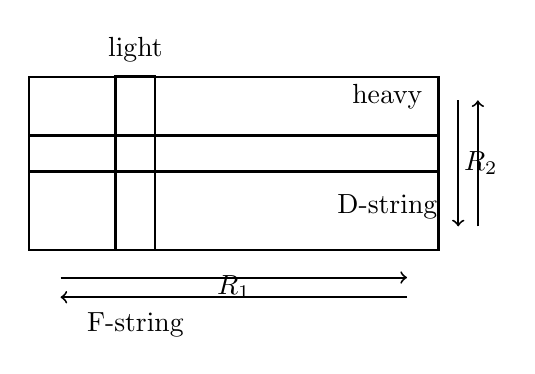
\begin{tikzpicture}[scale=1.0]
\draw[line width=0.9pt] (0,0) rectangle (5.2,2.2);
\node[below] at (2.6,-0.2) {\(R_1\)};
\node[right] at (5.4,1.1) {\(R_2\)};

\draw[->,line width=0.7pt] (5.45,1.9) -- (5.45,0.3);
\draw[->,line width=0.7pt] (5.7,0.3) -- (5.7,1.9);
\draw[->,line width=0.7pt] (0.4,-0.35) -- (4.8,-0.35);
\draw[->,line width=0.7pt] (4.8,-0.6) -- (0.4,-0.6);

\draw[line width=1.0pt] (1.1,0) -- (1.6,0) -- (1.6,2.2) -- (1.1,2.2) -- cycle;
\node at (1.35,2.55) {light};

\draw[line width=1.0pt] (0,1.45) -- (5.2,1.45);
\draw[line width=1.0pt] (0,1.00) -- (5.2,1.00);
\node at (4.55,1.95) {heavy};

\node at (1.35,-0.95) {F-string};
\node at (4.55,0.55) {D-string};
\end{tikzpicture}
\caption{Desde las direcciones no compactas, ambas configuraciones de membrana enrollada parecen cuerdas; sin embargo, las distintas escalas compactas hacen que una cuerda efectiva sea más ligera que la otra.}
\end{figure}

Esta es la versión geométrica de la historia de dualidad anterior. Al comprimir una dirección y estirar la otra, un objeto enrollado se vuelve más pesado y el otro más ligero, de modo que las funciones de las cuerdas F y D pueden intercambiarse.

\begin{classroomqa}
\audiencequestion{Si las direcciones compactas son cíclicas, ¿los objetos enrollados tienen anchura infinita? \lecturetimestamp{01:10:41}}
\lecturerresponse{No. Un círculo compacto tiene una circunferencia finita, aunque se pueda recorrer repetidamente sin llegar a un borde. La parte superior y la inferior del dibujo abierto en la pizarra representan el mismo punto, igual que los extremos de un intervalo pueden representar un mismo punto del círculo.}
\end{classroomqa}

\begin{figure}[htbp]
\centering
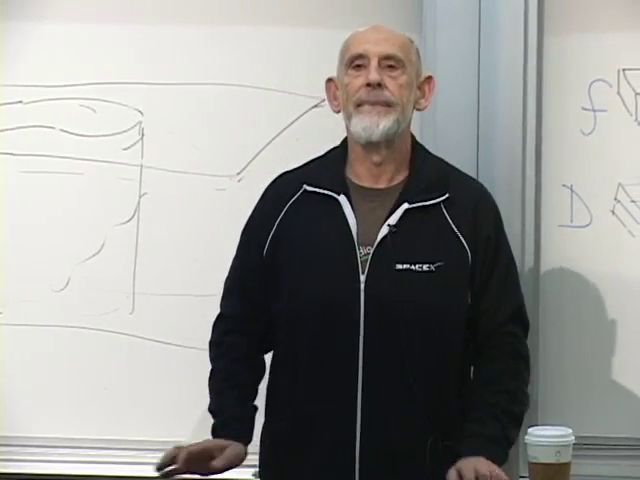
\includegraphics[width=0.78\textwidth]{lecture_01_figure_04.png}
\lectureframe{01:12:25.000}

\vspace{1em}

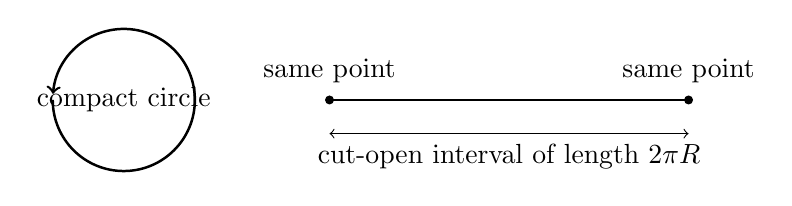
\begin{tikzpicture}[scale=0.95]
\draw[line width=0.9pt,->] (-3.7,0) arc[start angle=180,end angle=535,radius=0.95];
\node at (-2.75,0) {compact circle};
\draw[line width=0.9pt] (0.0,0) -- (4.8,0);
\fill (0.0,0) circle (0.06);
\fill (4.8,0) circle (0.06);
\draw[<->] (0.0,-0.45) -- (4.8,-0.45);
\node at (2.4,-0.75) {cut-open interval of length \(2\pi R\)};
\node[above] at (0.0,0.1) {same point};
\node[above] at (4.8,0.1) {same point};
\end{tikzpicture}
\caption{Un círculo compacto y su representación abierta en la pizarra. Al cruzar un extremo se vuelve a aparecer por el otro; en cambio, al avanzar en una dirección no compacta mientras se recorre el círculo se trazaría una hélice.}
\end{figure}

\begin{classroomqa}
\audiencequestion{¿Por qué la trayectoria compacta es un círculo y no una hélice? \lecturetimestamp{01:12:23}}
\lecturerresponse{En cada punto fijo de la dirección no compacta, la dirección compacta es un círculo. Solo aparece una hélice si se avanza en la dirección no compacta mientras se dan vueltas alrededor del círculo. El intervalo dibujado en la pizarra no es más que un círculo abierto por un corte, con sus dos extremos identificados.}
\end{classroomqa}

\begin{classroomqa}
\audiencequestion{¿Explica esta geometría por sí sola cómo una D-brana puede parecer un conjunto de cuerdas F cuando se la examina de cerca? \lecturetimestamp{01:12:49}}
\lecturerresponse{La conexión existe, pero no resulta evidente en esta imagen elemental; para verla hace falta un aparato geométrico más avanzado. El diagrama sirve para organizar la dualidad, no para derivar cada descripción de sus constituyentes microscópicos.}
\end{classroomqa}

\begin{classroomqa}
\audiencequestion{¿Podrían intercambiarse las direcciones compactas larga y corta al desplazarse por el espacio o con el paso del tiempo? \lecturetimestamp{01:13:35}}
\lecturerresponse{Cualquiera de las dos posibilidades se da en el modelo idealizado. Al aplastar un ciclo y expandir el otro, se intercambia cuál de las cuerdas enrolladas es ligera. Esta es otra razón por la que ``cuerda fundamental'' es solo un nombre: la descripción más conveniente puede cambiar de una región a otra o con el tiempo.}
\end{classroomqa}

\section{Idealización, puntos de simetría especial y el paisaje}

En el último tramo de la lección, Susskind se aleja de los elegantes ejemplos de dualidad y se pregunta qué nos dicen, y qué no, sobre el mundo real.

Primero, Susskind advierte que las dualidades que se pueden controlar con precisión son características de teorías supersimétricas muy idealizadas, en las que los bosones y los fermiones tienen masas exactamente iguales. Su analogía son las órbitas circulares de la mecánica newtoniana: se estudian primero porque son simétricas y matemáticamente manejables, no porque el movimiento real de los planetas se limite a círculos perfectos. Del mismo modo, las teorías de cuerdas supersimétricas son más fáciles de analizar porque son más simétricas que lo que parece ser la naturaleza.

Aun así, la idealización aporta información. Una órbita circular perfecta no representa un sistema planetario realista, pero muestra características que también se dan en órbitas menos simétricas. De modo parecido, los ejemplos supersimétricos muestran formas coherentes de compatibilizar la mecánica cuántica, la gravedad y la estructura microscópica. La formulación deliberadamente tajante de Susskind es que las teorías de cuerdas manejables no son, literalmente, la teoría de nuestro mundo; su valor reside en revelar fenómenos que probablemente también aparezcan en contextos menos simétricos y más difíciles de tratar.

\subsection{Un conjunto de piezas con muchos resultados posibles}

Las D-branas son solo parte del conjunto de piezas disponible. La lección también menciona flujos, orbifolds y orientifolds. Primero se elige una geometría compacta y luego qué branas y flujos ocupan sus ciclos. Incluso el sencillo sándwich cambia su física de dimensiones inferiores cuando se introduce una D2-brana flotante, dos o tres. Añadir o quitar estos elementos cambia las partículas, las interacciones y los parámetros efectivos.

Supongamos, siguiendo el recuento esquemático de la lección, que un espacio compacto de seis dimensiones tiene aproximadamente \(500\) ciclos y que en cada ciclo se puede elegir entre unas \(10\) configuraciones de branas enrolladas, flujos o estructuras relacionadas. Entonces, el número de construcciones crece como
\begin{equation}
N_{\mathrm{vacua}} \sim 10^{500}.
\end{equation}
La lógica del recuento de la lección es elemental:
\begin{equation}
10 \times 10 \times \cdots \times 10 = 10^{500}
\end{equation}
con \(500\) factores. La analogía con el ADN expresa la misma idea en términos más familiares:
\begin{equation}
N_{\mathrm{DNA}}(500)=4^{500}.
\end{equation}
Durante la comparación con el ADN, alguien del público comprueba que hay cuatro alternativas a lo largo de una hebra: A, C, G y T. La corrección refuerza el argumento, no lo cambia. Una lista corta de opciones locales, repetida muchas veces, produce una cantidad enorme de configuraciones globales. El exponente preciso no es lo importante, y Susskind califica \(10^{500}\) de una estimación demasiado baja, ya anticuada; lo importante es la proliferación combinatoria.

Así se completa la inversión de la expectativa reduccionista inicial. Una física de partículas complicada no tiene por qué surgir de reglas microscópicas complicadas. Puede surgir porque nuestro vacío es una configuración compleja de muchos elementos sencillos, igual que un organismo complejo puede codificarse mediante una secuencia construida a partir de cuatro bases.

\begin{classroomqa}
\audiencequestion{Una vez identificadas las descripciones equivalentes relacionadas por dualidad, ¿la información completa seleccionaría solo uno o unos pocos de estos vacíos posibles como descripciones de nuestro mundo? \lecturetimestamp{01:26:11}}
\lecturerresponse{Es de suponer que seleccionaría un conjunto restringido, pero muchos vacíos distintos podrían parecer extremadamente similares a las energías accesibles. El número citado para el paisaje pretende seguir siendo grande incluso tras identificar las descripciones duales, y los detalles irrelevantes de alta energía pueden funcionar como el ``ADN basura.''}
\end{classroomqa}

\subsection{Puntos simétricos y complejidad genérica}

Dentro del paisaje hay puntos con simetrías especiales. En la imagen geométrica, una configuración con razones de aspecto iguales,
\begin{equation}
R_1=R_2,
\end{equation}
hace que las dos descripciones del objeto enrollado sean igual de sencillas. En la analogía eléctrica--magnética, esto se representa esquemáticamente mediante
\begin{equation}
m_{\mathrm{monopole}}=m_e.
\end{equation}

\begin{figure}[htbp]
\centering
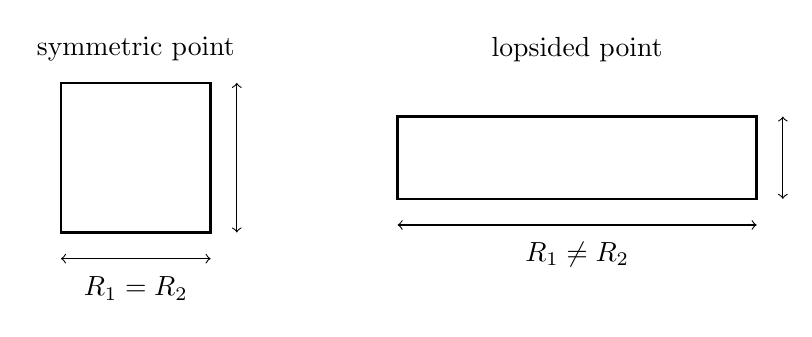
\begin{tikzpicture}[scale=0.95]
\draw[line width=0.9pt] (-4.5,-1.0) rectangle (-2.5,1.0);
\draw[<->] (-4.5,-1.35) -- (-2.5,-1.35);
\draw[<->] (-2.15,-1.0) -- (-2.15,1.0);
\node at (-3.5,1.45) {symmetric point};
\node at (-3.5,-1.75) {$R_1=R_2$};

\draw[line width=0.9pt] (0.0,-0.55) rectangle (4.8,0.55);
\draw[<->] (0.0,-0.9) -- (4.8,-0.9);
\draw[<->] (5.15,-0.55) -- (5.15,0.55);
\node at (2.4,1.45) {lopsided point};
\node at (2.4,-1.3) {$R_1\ne R_2$};
\end{tikzpicture}
\caption{Una compactificación con razones de aspecto iguales trata simétricamente las dos cuerdas enrolladas; una compactificación desequilibrada hace que una de las descripciones sea mucho más ligera que la otra.}
\end{figure}

\begin{classroomqa}
\audiencequestion{¿Hay vacíos en el paisaje donde la construcción sea mucho más sencilla porque las descripciones con cuerdas F y D coinciden? \lecturetimestamp{01:27:21}}
\lecturerresponse{Sí, hay puntos con simetrías especiales. Nuestro mundo no parece estar en uno de ellos: la partícula eléctrica conocida y un monopolo magnético no tienen la misma masa. Se desconoce por qué la naturaleza ocupa un punto desequilibrado.}
\end{classroomqa}

\editorialnote{La igualdad entre la masa del electrón y la del--monopolo es una característica esquemática de un modelo autodual adecuadamente protegido, no una predicción de la electrodinámica cuántica ordinaria sin supersimetría. Expresa la idea de punto de simetría de la lección, no una afirmación sobre el electrón observado.}

Susskind recuerda entonces una analogía de la teoría de la comunicación. Los códigos aleatorios pueden ser extraordinariamente buenos, mientras que los más fáciles de describir y decodificar tienen estructura matemática adicional y, históricamente, dieron peores resultados. Más adelante, la teoría de códigos encontró construcciones estructuradas muy eficaces, pero la analogía sigue en pie: todo lo que se puede nombrar o describir de manera concisa ocupa una región muy especial y de baja complejidad dentro del espacio completo de posibilidades. Del mismo modo, los vacíos de cuerdas más fáciles de calcular pueden ser atípicamente sencillos.

Por tanto, quizá convenga plantear otras preguntas. En lugar de exigir una descripción exacta de cada detalle microscópico de la compactificación, se puede preguntar qué características son comunes o genéricas en un conjunto amplio de posibilidades. Susskind presenta esto como un problema de investigación, no como una conclusión establecida, y rechaza los argumentos ideológicos como sustituto del cálculo.

\subsection{Cuestiones cosmológicas}

\begin{classroomqa}
\audiencequestion{¿Una dirección compacta de circunferencia enorme se distingue observacionalmente de una dirección infinita? ¿Y sabemos que nuestras tres grandes dimensiones espaciales son infinitas? \lecturetimestamp{01:30:03}}
\lecturerresponse{No sabemos si son infinitas. Una tres-esfera cerrada puede expandirse sin dejar de ser compacta. Las mediciones de una curvatura casi nula solo dan un límite inferior para el radio de curvatura, igual que medir un terreno casi llano puede acotar el tamaño de la Tierra sin demostrar que su superficie sea infinita. Solo detectar una curvatura o una identificación global permitiría determinar la escala finita.}
\end{classroomqa}

\begin{classroomqa}
\audiencequestion{Si el acoplamiento puede variar en el espacio en el modelo idealizado, ¿cómo podría producirse esa variación en el mundo real? \lecturetimestamp{01:32:43}}
\lecturerresponse{No como la variación suave sin restricciones del ejemplo simétrico. La posibilidad realista que se analizará más adelante es una variación mediante transiciones discretas entre regiones con leyes efectivas distintas. Que se produzcan tales saltos es una cuestión cosmológica.}
\end{classroomqa}

\editorialnote{Esta respuesta debe entenderse como un anticipo de la lección sobre vacíos de flujo y transiciones entre dominios, no como un teorema general que prohíba todo campo escalar con variación suave. Las observaciones restringen fuertemente las variaciones de los acoplamientos adimensionales, mientras que los mecanismos de estabilización determinan si quedan moduli continuos disponibles en un modelo dado.}

La grabación no conserva la última pregunta del público. La respuesta que sí se conserva dice que el fenómeno propuesto puede darse en algunos tipos de agujeros negros, pero no en el horizonte de un agujero negro ordinario de Schwarzschild, que para un observador en caída libre es localmente un lugar corriente. Como no se puede reconstruir la pregunta con fiabilidad, no se atribuye al intercambio ninguna afirmación más específica.

\section{De los ladrillos a una red de descripciones}

La esperanza de que las capas más profundas de la física deban ser más sencillas ha resultado frágil. En la bosonización en \(1+1\) dimensiones, una misma teoría puede organizarse en torno a fermiones o a bosones, y el fermión reaparece como un kink. En la electrodinámica cuántica, el acoplamiento débil y el fuerte intercambian las funciones descriptivas del electrón y el monopolo magnético. En la teoría de cuerdas, las cuerdas F y D reproducen el mismo patrón, y en la teoría de branas pares el acoplamiento fuerte lleva aún más lejos esta idea: se expande una dirección compacta, las D0-branas se convierten en estados de momento de Kaluza--Klein y las cuerdas efectivas se reinterpretan como membranas enrolladas en una geometría de dimensiones superiores. Por tanto, la teoría cuántica de campos y la teoría de cuerdas modernas no ofrecen una respuesta única y definitiva a la pregunta ``¿cuáles son los ladrillos y cuáles las casas?'' Ofrecen una red de descripciones, cada una eficiente en su propio régimen, junto con un vasto paisaje de construcciones posibles cuyo resultado genérico es la complejidad, no la simplicidad.
